\subsection{Overordnet system}

På figur 2.2, på næste side, beskrives hvilke blokke der er koblet sammen samt hvilke
signaler de sender til hinanden.

\begin{figure}[H]
\centering
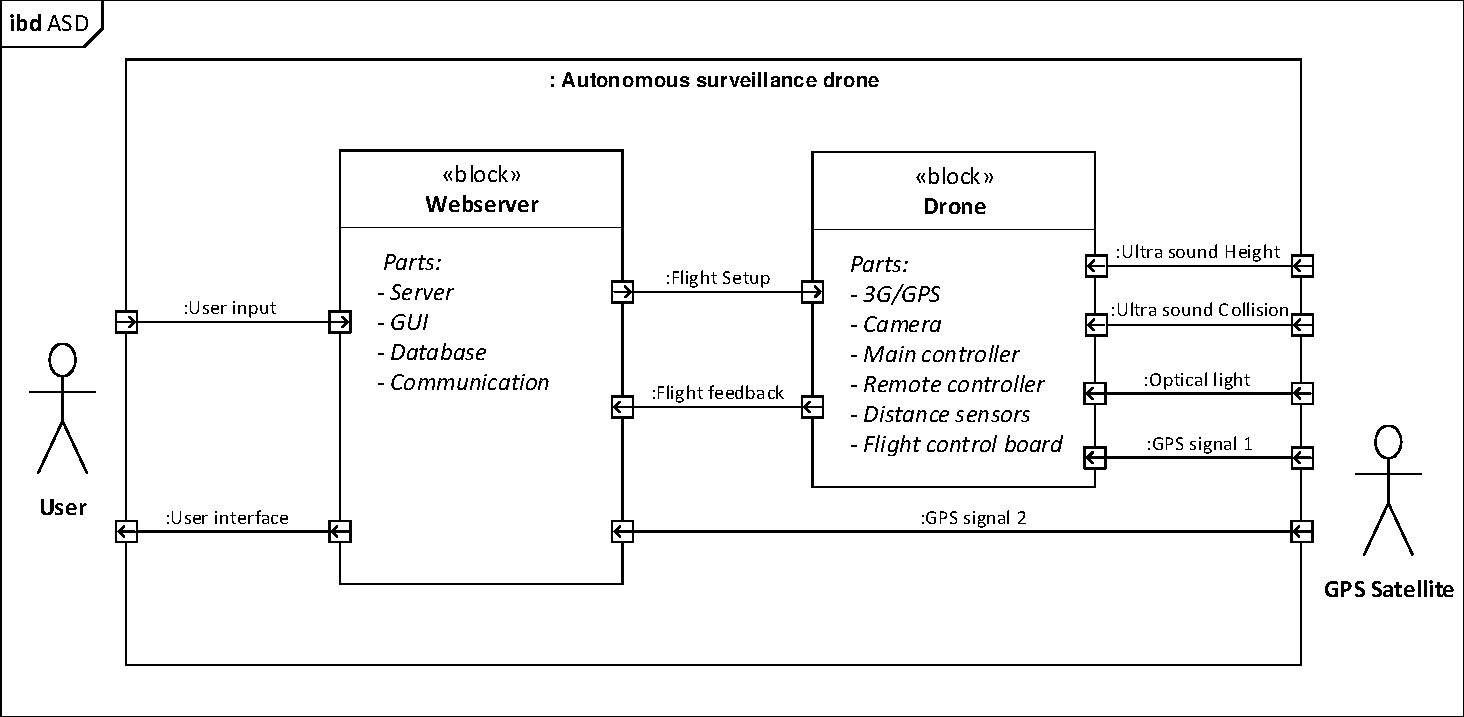
\includegraphics[width=1\textwidth]{Billeder/IBD/ibd1_overordnet.pdf}
\caption{ibd - overordnet}
\label{fig:ibd_overordnet}
\end{figure}

\begin{table}[H]
	\centering
		\begin{tabular}{|p{2.5 cm}|p{5.5 cm}|p{2.5 cm}|p{2.5 cm}|} 
		\hline
			\textbf{Signal navn} 	& \textbf{Signal beskrivelse}		& \textbf{Out} 				& \textbf{In}     \\ \hline
			User input 			& Via \textit{webapplication} opsætter bruger ny flyvning eller undersøger tidligere & Bruger 		& Webapplication.			    \\ \hline
			User interface 		& Via GUI kan bruger se hvad der sker i\textit{webapplication}.	& Webapplication.			& Bruger.				\\ \hline
			Flight setup		& Fra \textit{webapplication} sendes flyveopsætningen til dronen.	& Webapplication.	& Dronen.	\\ \hline
			Flight feedback		& Informationer fra dronen til \textit{webapplication}.	& 	Dronen.		& Webapplication.			    \\ \hline
			GPS signal 1		& GPS signal fra GPS-satellitter.	& GPS-satellit.			& Dronen.				\\ \hline
			GPS signal 2		& GPS signal fra GPS-satellitter.	& GPS-satellit.				& Webapplication.	\\ \hline  
		\end{tabular}
	\caption{Forbindelser IDB 1}
	\label{tab:IDB1}
\end{table}

